



\chapter{The physics of magnetism}

\noindent
BACKGROUND: Read chapters on magnetism from your favorite college  physics book for review.
\vskip 6pt


Paleomagnetism is the study of the magnetic properties of rocks. 
It is one of the most broadly applicable  disciplines in
geophysics,
having uses in diverse fields such as geomagnetism, tectonics,
paleoceanography, volcanology, paleontology, and sedimentology.  
  Although the potential applications are varied, the
fundamental techniques are remarkably uniform.  Thus, a grounding in the
basic tools 
of paleomagnetic data analysis can open doors  to 
many of these applications.  One of the underpinnings of paleomagnetic
endeavors is the relationship between the magnetic properties of rocks
and the Earth's magnetic field.  

In this chapter we will review the basic physical principles behind magnetism:  what are magnetic fields, how are they  produced and how are they measured?   Although many find a discussion of scientific units boring,  much confusion arose when paleomagnetists switched from   ``cgs''  to the Syst\`eme International (SI) units and mistakes abound in the literature.  Therefore,  we will explain both unit systems and look at how to  convert successfully between them.    There is a review of essential mathematical tricks in Appendix~\ref{app:definitions} to which the reader is referred for help. 


\index{magnetic!field!definition}%
\index{magnetic!units!SI}%
\section{What is a magnetic field?}
\label{sect:H}


Magnetic fields, like gravitational fields, cannot be seen or touched.  We
can feel the pull of the Earth's gravitational field on ourselves and the
objects around us, but we do not experience magnetic fields in such a
direct way.  We know of the existence of magnetic fields by their effect
on objects such as magnetized pieces of metal, naturally magnetic
rocks such as lodestone, or temporary magnets such as copper coils that carry
an electrical current.  If we place a magnetized needle on a cork in a
bucket of water, it will slowly align itself with the local magnetic field.
Turning on the current in a copper wire can make a nearby compass needle jump.
Observations like these led to the development of the concept of 
magnetic fields.

\begin{figure}[htb]
 \centering   \includegraphics[width=10cm]{EPSFiles/wire.eps} 
\caption{ a) Distribution of iron filings on a flat sheet pierced by a wire
carrying a current $i$.   [From Jiles, 1991.]  b) Relationship of magnetic field  to current for straight wire. }
\label{fig:filings}
\end{figure}
 \nocite{jiles91}


%\customlink{filings}


Electric currents make magnetic fields, so we can define what is meant by a
\index{magnetic!field!definition}%
``magnetic field'' in
 terms of the
electric current that generates it.
Figure~\ref{fig:filings}a is a picture of what
happens  when we pierce a flat sheet with a wire carrying
a current $i$.  When iron filings are sprinkled on the sheet, 
the filings line up
with the magnetic field produced by the current in the wire.  A
loop tangential to the field is shown
in Figure~\ref{fig:filings}b, which  illustrates the 
\index{right-hand rule}%
{\it right-hand rule} (see inset to Figure~\ref{fig:filings}b). If your right thumb points in the direction
of  (positive) current flow (the direction opposite to the flow of the electrons), your fingers  will curl in the direction of the magnetic
field.  

  The magnetic field $\H$ points at right angles to both the direction of
current flow and to the radial  vector $\mathbf{r}$ in Figure~\ref{fig:filings}b.  The 
\index{magnetic!field!magnitude}%
magnitude of
$\H$  (denoted $H$)  is proportional to the strength
of the current $i$. In the simple case illustrated in
Figure~\ref{fig:filings}b  the magnitude of $\H$ is given by 
\index{Amp\`ere's law}%
Amp\`ere's law:
$$
\ H = {i \over{2 \pi r}},
$$

\noindent where $r$ is the length of the vector $\mathbf{r}$.  So, now we know  the units of $H$:  Am$^{-1}$.

 Amp\`ere's Law in its most general form is  one of 
\index{Maxwell's equations}%
Maxwell's
equations of electromagnetism:   in a steady electrical field,
 ${\bf \nabla} \cross \H = \J_f$, where $\J_f$ is
the 
\index{electric!current density}
electric current density (see Section~\ref{app:nabla} in the appendix for review of the $\nabla$ operator).  
In words, the
 curl (or circulation)
 of the magnetic field is
equal to the current density.  The origin of the term ``curl'' for the 
cross product of   the gradient operator with a vector field 
is suggested in Figure~\ref{fig:filings}a  in which the iron filings
seem to curl around the wire.  
 
\index{magnetic!moment}%
\section {Magnetic moment}
\label{sect:moment}

%\customlink{magnetic_moment}



An electrical current in a wire produces a magnetic field
that ``curls'' around the wire.  If we bend the wire into a 
\index{electric!current loop}
loop with an  area $\pi r^2$ that carries
a current $i$ (Figure~\ref{fig:moment}a), the current loop would
 create  the magnetic field shown by pattern of the iron filings.  This magnetic field is that same as the field that would be produced by a permanent magnet. We can quantify the strength of that hypothetical magnet in terms of a {\it magnetic moment}  $\m$ (Figure~\ref{fig:moment}b).  The magnetic moment is  created by a current $i$ and  also depends on the area of the current loop (the bigger the loop, the bigger the moment).  Therefore,  the magnitude of the moment can by quantified by  $m = {i {\pi r^2}}$. The moment created by a set of  loops (as shown in Figure~\ref{fig:moment}c) would be the sum of the $n$ individual loops, i.e.:

\begin{equation}
 m = n{i {\pi r^2}}.
 \label{eq:moment}
 \end{equation}

\noindent  So, now we know the units of $\m$:   Am$^2$.    In nature, magnetic moments are carried by magnetic minerals the most common of which are magnetite and hematite (see Chapter 6 for details). 

   \begin{figure}[htb]
\centering  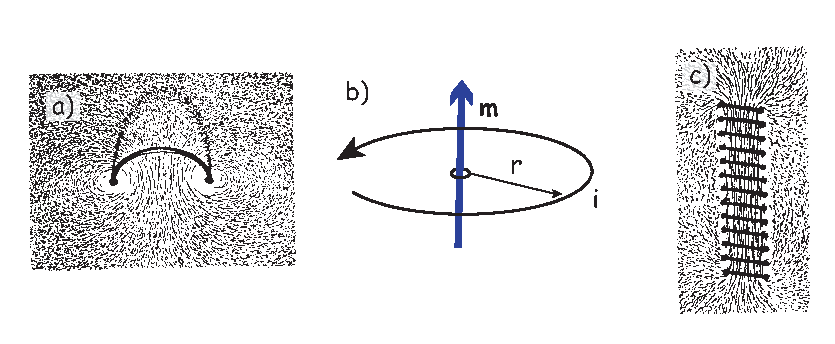
\includegraphics[width=14 cm]{EPSfiles/moment.eps}
\caption {a) Iron filings show the magnetic field generated by current flowing in a loop. b) A current loop with current $i$ and area $\pi r^2$  produces a magnetic moment $\mathbf{m}$.  c) The magnetic field of loops arranged as a solenoid  is the sum of the contribution of the individual loops.  [Iron filings pictures from Jiles, 1991.] }
\label{fig:moment}
\end{figure}
\nocite{jiles91}
  
  
\index{magnetic!flux}%
\section{Magnetic flux}
\label{sect:flux}

The magnetic field is a vector field because at any point it has both direction and magnitude.  Consider the field of the bar magnet in Figure~\ref{fig:barmagnet}a.  The direction of the field at any point is given by the arrows while the strength depends on how close the field lines are to one another.   The magnetic field lines represent  
\index{magnetic!flux}%
{\it magnetic flux}.      The density of flux lines is one measure of the strength of the
magnetic field:  the magnetic induction $\B$.  
 
        \begin{figure}[htb]
\centering  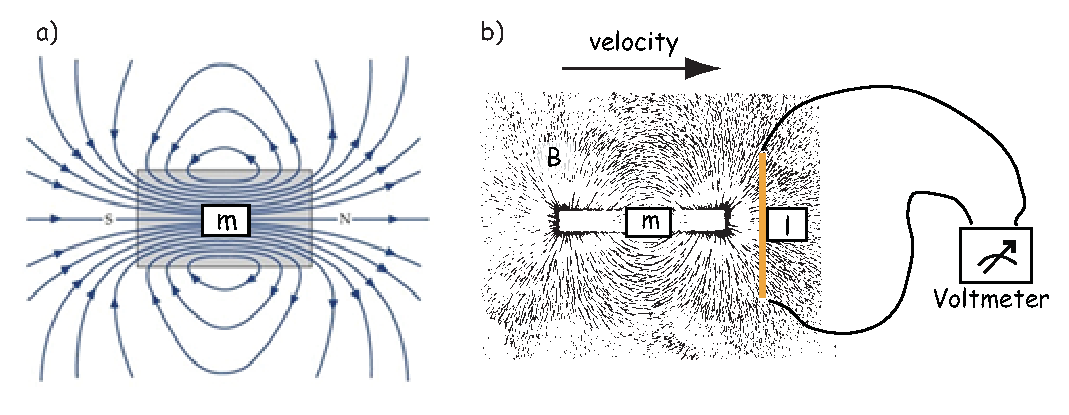
\includegraphics[width=14 cm]{EPSfiles/barmagnetfield.eps}
\caption {a) A magnetic moment $\mathbf{m}$  makes a vector field $\B$.  The lines of flux are represented by the arrows.   [Adapted from  Tipler, 1999.] b) A magnetic moment $\mathbf{m}$  makes a vector field $\B$ made visible by the iron filings.  If this field moves with velocity $\mathbf{v}$, it  generates a voltage $V$ in an electrical conductor of length $l$.   [Iron filings picture from Jiles, 1991.]}
\label{fig:barmagnet}
\end{figure}
 \nocite{jiles91,tipler99}

Just as the motion of electrically charged particles in a wire (a current) create a magnetic field 
\index{Amp\`ere's law}%
(Amp\`ere's Law), the motion of a magnetic field creates electric currents in nearby wires.   The stronger the magnetic field, the stronger the current in the wire.  
\index{magnetic!induction}
We can therefore measure the strength of the magnetic induction (the density of magnetic flux lines)  by moving a conductive wire through the magnetic field (Figure~\ref{fig:barmagnet}b).  

Magnetic induction can be thought of as something that creates a potential difference with voltage $V$ in a conductor of length $l$ when the conductor moves relative to the magnetic induction $B$ with velocity $\mathbf{v}$ (see Figure~\ref{fig:barmagnet}b): $ V=vlB$.    
From this we can derive the units of magnetic induction:  the 
\index{tesla}%
tesla (T).   One tesla is the magnetic induction that generates  a potential of one volt in a conductor of length one meter when moving at a rate of one meter per second.   So now we know the units of $\B$:   V $\cdot$ s $\cdot$ m$^{-2}$ = T.


\index{magnetic!flux density}
Another way of looking at $\B$ is that if magnetic induction is the density of magnetic flux lines, it must be  the flux $\Phi$ per unit area.  So an increment of flux $d\Phi $ is the field magnitude $B $ times the increment of area $dA$.  The area here is the length of the wire $l$ times its displacement $ds$ in time $dt$.  The instantaneous velocity is $dv = ds/dt$ so $d\Phi = B dA$ and the rate of change of flux is:

\begin{equation}
{d\Phi \over {dt} } = \bigl( {ds\over {dt}} \bigr) B l = vBl = V.  
\label{eq:faraday}
\end{equation}

Equation~\ref{eq:faraday} is known as 
\index{Faraday's Law}
Faraday's law and in its most general form is the fourth of 
\index{Maxwell's equations}%
Maxwell's equations.    We see from Equation~\ref{eq:faraday} that the units of magnetic  flux must be  a  volt-second which is a unit in its own right: the 
\index{weber}%
weber (Wb). The weber is defined as the amount of magnetic flux which, when
passed through a one-turn coil of a conductor    
carrying a current of one ampere, produces an electric potential of one volt. 
This definition suggests a means to measure the strength of magnetic 
induction and is the basis of the 
\index{fluxgate magnetometer}%
``fluxgate'' magnetometer.

\index{magnetic!energy}%
\section {Magnetic energy}
\label{sect:Me}

A magnetic moment $\m$  in the presence of a magnetic field $\B$ 
has a
\index{magnetic!energy!magnetostatic}%
 {\it magnetostatic energy} ($E_m$) associated with it.  This  energy tends to align compass needles with the magnetic field (see Figure~\ref{fig:compass}).  
$E_m$ is given by $-\m \cdot \B$  or $-m B  \cos \theta$ where $m$ and
$B$ are the magnitudes of $\m$ and $\B$, respectively (see Section~\ref{app:vecmult} in the appendix for review of vector multiplication). Magnetic energy has units of joules and is at a minimum when $\m$ is aligned with $\B$.

 \begin{figure}[htb]
 \centering 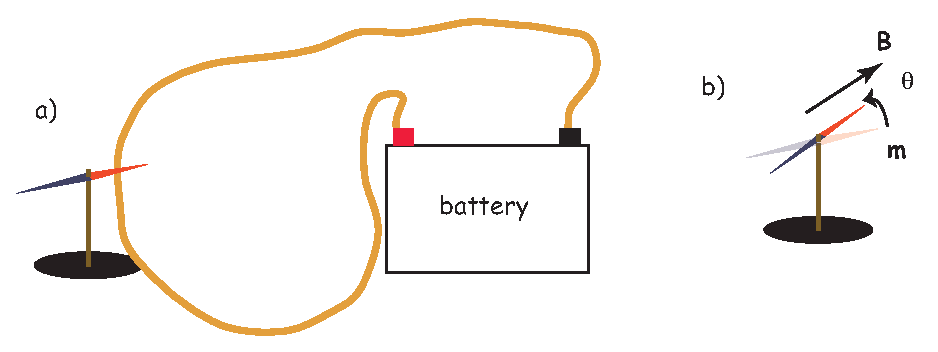
\includegraphics[width=12 cm]{EPSfiles/compass.eps}
\caption {The magnetic moment $\m$  of, for example, a compass needle, will tend to align itself with a magnetic field $\B$.  a) Example of when the field is produced by a current in a wire.  b) The aligning energy is the magnetostatic energy which is greatest when the angle $\theta$ between the two vectors of the magnetic moment $\m$ and the magnetic field $\B$  is at a maximum.   }
\label{fig:compass}
\end{figure}

  
 \index{magnetization}%
 \index{magnetic!susceptibility}
\section {Magnetization and magnetic susceptibility}
\label{sect:mag}

{\it Magnetization} $\M$
 is a normalized  moment (Am$^2$).  We will use the symbol $\M$ for volume normalization  (units of Am$^{-1}$) or  $\Omega$ for mass normalization (units of  Am$^2$kg$^{-1}$).    Volume normalized magnetization therefore has the same units as $\H$, implying that there  is a current somewhere, even in permanent magnets.  
In the classical view (pre-quantum mechanics), sub-atomic charges such as protons and electrons 
can be thought of as tracing out tiny circuits and behaving as
tiny magnetic moments. They respond to external magnetic fields and give
rise to an induced magnetization.  The relationship
between the magnetization induced in a material $\M_I$ and the external field $\H$ is defined as:

\beq
\M_I =\chi_b \H.
\label{eq:chi}
\eeq

\noindent The parameter $\chi_b$ is known as the 
 \index{magnetic!susceptibility!bulk}%
 {\it bulk magnetic susceptibility} of
the material; it can be a 
complicated function of orientation, temperature, state of stress, time scale of observation
and applied field, but is often treated as  a scalar.   Because $\M$ and $\H$ have the same units, $\chi_b$ is dimensionless.  
In practice, the magnetic response of a substance to an applied field can be normalized by volume (as in Equation~\ref{eq:chi}) or by mass
or not normalized at all.  We will use the symbol $\kappa$ for mass normalized susceptibility and $K$ for the raw measurements (see Table~\ref{tab:units}) when necessary.

Certain materials can produce magnetic fields in the absence of
external magnetic fields (i.e., they are permanent magnets).  As we shall
see in later chapters, these so-called ``spontaneous''
 magnetic moments are also the result of 
spins  of electrons which, in some crystals, act
in a coordinated fashion, thereby producing a net magnetic field. 
The resulting 
\index{magnetization!spontaneous}
spontaneous magnetization can be fixed by various mechanisms and can
preserve records of ancient magnetic fields.  This 
\index{magnetization!remanent}
 {\it remanent magnetization} forms the basis of the field of paleomagnetism
and will be discussed at length in subsequent chapters. 
 
 
\section {Relationship of $\B$ and $\H$}
\label{sect:BvH}

 $\B$ and $\H$ are closely related and in  paleomagnetic practice, both $\B$ and $\H$ are referred to as the 
``magnetic field''.  Strictly
speaking, $\B$ is the induction and $\H$ is the field, but the distinction
is often blurred.  The relationship between $\B$ and $\H$ is given by: 

\beq
\B = \mu (\H + \M).
\label{eq:B}
\eeq

\noindent where $\mu$ is a physical constant known as 
{\it the permeability}.   In a vacuum, this is the
\index{magnetic!permeability of free space}
permeability of free space, $\mu_o$. 
 In the SI system, 
$\mu$ has dimensions of henries per meter and $\mu_o$ is

$4\pi \cross 10^{-7} \hbox{H} \cdot \hbox{m}^{-1}$.  In most cases of paleomagnetic interest, we are outside the magnetized body so $\M=0$ and $\B=\mu_o \H$.   

\index{magnetic!units!cgs}%
\section {A brief tour of magnetic units in the cgs system}

So far, we  have derived magnetic units in terms of the 
Syst\` eme International (SI).  In practice, you will
notice that  people frequently use what are known as cgs units, based on centimeters, grams and seconds.  You may wonder why any fuss would be made over using meters as opposed to centimeters because the conversion is trivial.  With magnetic units, however, the conversion is far from trivial and has been the source of confusion and many errors.    So, in the interest of clearing things up,  we will briefly outline the cgs approach to magnetic units. 

\begin{figure}[htb]
 \centering 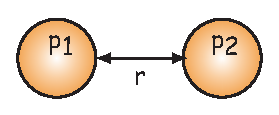
\includegraphics{EPSfiles/pp.eps}
\caption{The force between two magnetic monopoles $p_1,p_2$ is $p_1p_2\over{r^2}$. \hfill}
\label{fig:pp}
\end{figure} 

\eject
The derivation of magnetic units in cgs is entirely different from SI.  The approach we will take here follows that of 
\index{Cullity, B.D.} \nocite{cullity72}
Cullity (1972).  We   
start with the concept of a 
\index{magnetic!pole strength}
magnetic pole with strength $p$ instead of with current loops as we did for  SI units.    
We will consider   the force between two poles $p_1,p_2$ (see Figure~\ref{fig:pp})  \index{Coulomb's Law}% 
Coulomb's law.   This
states that the force between two charges ($q_1,q_2$) is:
  
\begin{equation}
 F_{12} = k { {q_1q_2}\over {r^2} },
 \label{eq:coulomb}
\end{equation}
 \noindent
 where $r$ is the distance between the two charges.  In cgs units, the proportionality constant $k$ is simply unity, whereas in SI units it is ${1\over {4\pi \epsilon_0}}$ where $\epsilon_0 = { {10^7}\over {4\pi \hbox{c}^2} }$ and $c$ is the speed of light in a vacuum (hence $\epsilon_0= 8.859 \cdot 10^{-12}$ AsV$^{-1}$m$^{-1}$).  [You can see why many people really prefer cgs but we are not allowed to publish in cgs in most of geophysical journals so we just must grin and bear it!]   
 
 For magnetic units, we use pole strength $p_1, p_2$ in units of
 \index{electrostatic unit}
{\it electrostatic units} or esu, so Equation~\ref{eq:coulomb} becomes
 $$
 F =  { {p_1p_2}\over {r^2} }.
 $$

\noindent Force in cgs is in units of dynes (dyn),  so
$$
  F = 1  \hbox{ dyn} = { {1 \hbox{g cm }} \over {s^2} } = {{1 \hbox{ esu}^2} \over {cm^2} },
  $$
\noindent so 1 unit of pole strength  is rather awkwardly 1 gm$^{1/2}$ cm$^{3/2}$ s$^{-1}$.   Of course there are no isolated magnetic poles in nature, only dipoles, but the concept of a unit of pole strength lies at the heart of cgs magnetic units.  

A magnetic pole, as an isolated electric charge, would create a 
\index{magnetic!induction}
magnetic induction $\mu_oH$ in the space around it.  One unit of field strength (defined as one 
\index{oersted}
{\it oersted}  or Oe) is the unit of field strength that exerts a force of one dyne on a unit of pole strength.   The related induction ($\mu_oH$) has units of gauss or G. 

The relationship between force, pole and magnetic field is written as:

$$
F = p\mu_oH.
$$
\noindent So, a pole  with one pole strength, placed in a one Oe field is acted on by a force of one dyne.  This is the same force that it would experience if we placed the pole one centimeter away from another pole with one pole strength.    Hence, the strength of the field produced by  this monopole must be one oersted at one centimeter distance, and decrease proportional to  $1/r^2$.  

Returning to the lines of force idea developed for magnetic fields earlier, let us define the oersted to be the magnetic field which would produce an induction with  one unit of induction per square centimeter.  Imagine a sphere with a radius $r$ surrounding the magnetic monopole.  The surface area of such a sphere is $4\pi r^2$.   When the sphere is a unit sphere ($r=1$) and the field strength at the surface is 1 Oe, then there must be  a magnetic flux of $4\pi$ units of induction passing through it.    


You will have noticed the use of the
\index{magnetic!permeability of free space}
 permeability of free space $\mu_o$ in the above treatment -- a parameter missing in  many books and articles using the cgs units.  The reason for this is that $\mu_o$ is unity in cgs units and simply converts oersteds ($\H$) to  gauss ($\B=\mu_o\H$).  Therefore in cgs units, $B$ and $H$  are used interchangeably.  We inserted it in this derivation to remind us that there IS a difference and that the difference becomes very important when we convert to SI because $\mu_o$ is not unity, but $4\pi$ x 10$^{-7}$!  For conversion between commonly used cgs and SI paramters, please refer to Table~\ref{tab:units}.

Proceeding to the notion of magnetic moment, from a cgs point of view, we start with a magnet of length $l$ with two poles of strength $p$ at each end.    Placing the magnet in a field $\mu_o\H$, we find that it experiences a torque $\Gamma$ proportional to $p, l$ and  $\H$ such that

\begin{equation}
\Gamma= pl \cross \mu_o\H.
\label{eq:torque}
\end{equation}

\noindent  Recalling our earlier discussion of magnetic moment, you will realize that $pl$ is simply the magnetic moment $m$.   This line of reasoning also makes clear why it is called a ``moment''.   The units of torque are energy, which are ergs in cgs, so the units of magnetic moment are technically erg per gauss.  But because of the ``silent'' $\mu_o$ in cgs, magnetic moment is most often defined as erg per oersted  We therefore follow convention and define the
\index{electromagnetic unit (emu)!derivation}
 ``electromagnetic unit'' (emu) as being one erg $\cdot$ oe$^{-1}$. [Some use emu to refer to the magnetization (volume normalized moment, see above), but this is incorrect and a source of a lot of confusion.]  


\index{magnetic!units!conversion}%
{%\hoffset -1in
%\vskip -.3in
\begin{table}[h!tb]
\caption{Conversion between SI and cgs units.}
\label{tab:units}
\begin{tabular}{lllll}
\hline
 Parameter &   SI unit&  cgs unit&
 Conversion \\
\hline
 Magnetic moment  ($\m$) & Am$^2$ & emu &  1 A m$^2$ = 10$^3$ emu \\
Magnetization\\
\hskip 1em by volume  ($\M$) & Am$^{-1}$ &  emu cm$^{-3}$ & 1 Am$^{-1}$ = 10$^{-3}$ emu cm$^{-3}$\\
\hskip 1em by mass ($\Omega$)&Am${^2}$kg$^{-1}$& emu gm$^{-1}$ & 1 Am$^2$kg$^{-1}$ = 1 emu gm$^{-1}$\\
Magnetic Field ($\H$) & Am$^{-1}$ & Oersted (oe) & 1 Am$^{-1}$ = 
4$\pi$ x 10$^{-3}$ oe \\
Magnetic Induction  ($\B$) & T  & Gauss (G) & 1 T =
10$^4$ G \\
Permeability \\
of free space ($\mu_o$)& Hm$^{-1}$  & 1 & 4$\pi$ 
x $10^{-7}$ Hm$^{-1}$ = 1  \\
Susceptibility \\
 \hskip 1em total (K:$\m \over \H$)  &m$^3$ & emu oe$^{-1}$ & 1 m$^3 =
{{10^6}\over {4\pi }}$ emu oe$^{-1}$\\
 \hskip 1em by volume (  $\chi$: $\M \over \H$) & - & emu cm$^{-3}$ oe$^{-1}$ & 1 S.I.  = ${1\over
{4\pi}}$ emu cm$^{-3}$ oe$^{-1}$\\
 \hskip 1em by mass ($\kappa$:${\m \over m}\cdot {1\over \H}$)  & m$^3$kg $^{-1}$
& emu g$^{-1}$ oe$^{-1}$ & 1 m$^3$kg$^{-1}$ = ${{10^3}\over {4 \pi}}$emu 
g$^{-1}$ oe$^{-1}$ \\
\hline
\end{tabular}

{ 1 H = kg m$^2$A$^{-2}$s$^{-2}$}, { 1 emu = 1 G cm$^3$},{ $B = \mu_o H$ (in vacuum)},
{ 1 T = kg A$^{-1}$ s$^{-2}$} 
\end{table}
}



 

\index{magnetic!potential}%
\section{The magnetic potential }
\label{sect:potential}

An isolated electrical charge produces an electrical field that
begins at the source  
(the charge) and spread (diverge) outward (see Figure~\ref{fig:divergence}a).  
Because there is no return flux to an oppositely charged ``sink'',  there is a net flux out of the dashed box shown in the figure.  The 
{\it divergence}  of the electrical field is defined as ${\bf \nabla} \cdot \E$ which quantifies the net flux (see Appendix~\ref{app:nabla} for more).   In the case of the field around an electric charge, the divergence is non-zero.

Magnetic fields are different from electrical fields in that there is no
equivalent to an isolated electrical charge; there are only pairs of
``opposite charges'' -- magnetic 
\index{magnetic!dipole}%
{\it dipoles}. Therefore, any line of flux starting at one magnetic pole, returns to its sister pole and there is no net flux out of the box shown in Figure~\ref{fig:divergence}b;  the magnetic field has no divergence (Figure~\ref{fig:divergence}b).  This property of magnetic fields is  another
\index{Maxwell's equations}%
of Maxwell's equations: ${\bf \nabla} \cdot \B = 0$.

\begin{figure}[htb]
 \centering 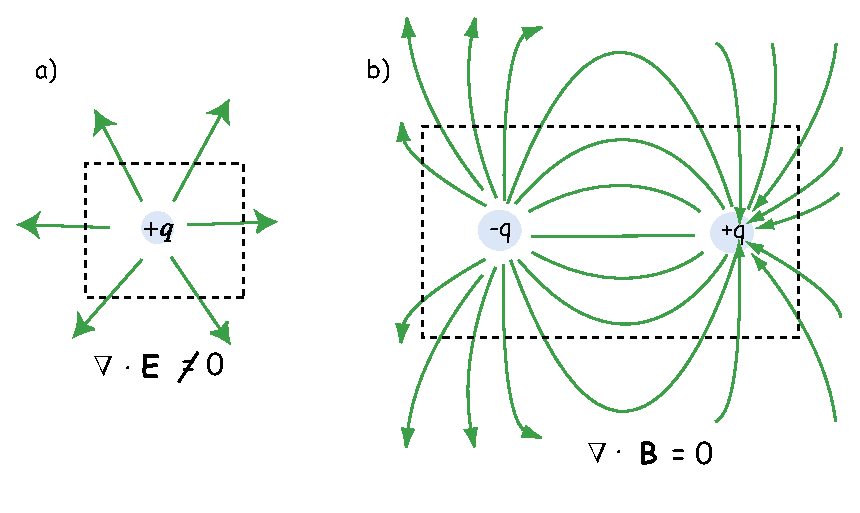
\includegraphics[width=12 cm]{EPSfiles/divergence.eps}
\caption{a) An electric charge produces a field that diverges out from the source.   There is a net flux out of the dashed box, quantified by the divergence ($\nabla \cdot \E$), which is  is proportional to the magnitude of the  sources inside the box.  b) There are no isolated magnetic charges, only dipoles.  Within any space (e.g., the dashed box)  any flux line that goes out must return.  The divergence of such a field is zero, i.e., $\nabla \cdot \B = 0$.  }
\label{fig:divergence}
\end{figure}


   In the special case away
from electric currents and magnetic sources (so $B=\mu_oH$),  
the magnetic field can be written as the gradient
of a scalar field
that is known as the
\index{magnetic!potential}%
 {\it magnetic potential},  $\psi_m$, \ie  

$$
\H = - {\bf \nabla} \psi_m.
$$



The presence of a magnetic moment $\m$ creates a 
magnetic field which is the gradient of some scalar
field.  To gain a better intuitive feel about the relationship between scalar fields and their gradient vector fields, see Appendix~\ref{app:nabla}.   Because the divergence of the magnetic field is zero, by definition, the divergence of the gradient of the scalar field is also  zero, or  $\nabla^2 \psi_m =0$.   The operator $\nabla^2$ is called the Laplacian and $\nabla^2 \psi_m= 0$ is 
\index{Laplace's equation}
{\it Laplace's equation}.  This  will be the starting point for spherical harmonic analysis of the geomagnetic field discussed briefly in Chapter  2.  



The curl of the magnetic field $(\nabla \cross \H)$
depends on the current density and is not always zero and magnetic fields cannot generally be  represented as the gradient of a scalar field.  Laplace's equation is only valid outside the magnetic sources and away from currents.   

\index{magnetic!potential}%
So what is this magnetic potential and how does it relate to the magnetic moments that give rise to the magnetic field?  Whatever it is, it has to satisfy Laplace's equation, so we turn to solutions of Laplace's equation for help.  One solution is to define the magnetic potential $\psi_m$ as a
function of  the vector $\mathbf{r}$ with radial distance $r$ and the angle $\theta$  from the moment.
Given a 
\index{dipole!moment}%
{\it dipole moment} $\m$, a solution to Laplace's equation  is:

\beq
\psi_m = {{\m\cdot \mathbf{r}}\over {4\pi r^3}}= {{m\cos \theta}\over {4\pi r^2}}.
\label{eq:Vm}
\eeq

\noindent You can verify this by making sure that$\nabla^2 \psi_m =0$.  

The radial and tangential components of $\H$ at P (Figure~\ref{fig:mH}) then would be:

$$
H_r =- {{\partial \psi_m \over {\partial r}}} = {1\over
{4\pi}}{{2m \cos\theta}\over {r^3}},
$$
\noindent and 
\begin{equation}
H_{\theta} = - {1\over r}{{\partial \psi_m}\over {\partial \theta}} = {{m \sin
\theta}\over{4\pi r^3}},
\label{eq:HrHt}
\end{equation}
respectively. 

\begin{figure}[h!tb]
 \centering 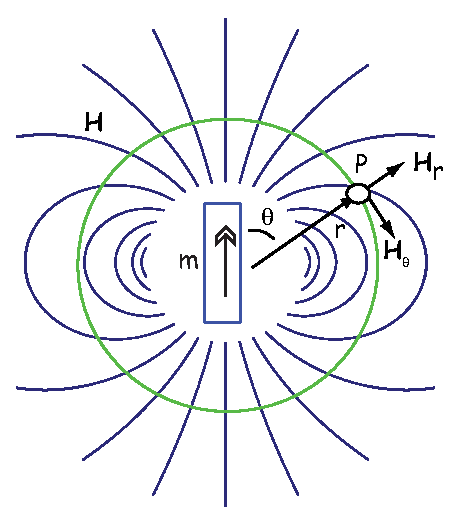
\includegraphics[width=6 cm]{EPSfiles/mH.eps}
\caption
{Field $\H$ produced at point P by a magnetic  moment $\m$. $\H_r$
and $\H_{\theta}$ are the radial and tangential fields respectively.}
\label{fig:mH}
\end{figure}



\section{Origin of the geomagnetic field}

Measurement and description of the geomagnetic field and its spatial and temporal variations constitute one
of the oldest geophysical disciplines. However, our ability to describe the field far exceeds our understanding
of its origin. All plausible theories involve generation of the geomagnetic field within the fluid outer core
of the Earth by some form of magnetohydrodynamic dynamo. Attempts to solve the full mathematical
complexities of magnetohydrodynamics  succeeded only in 1995 (Glatzmaier and Roberts, 1995).  \nocite{glatzmaier95}

Quantitative treatment of magnetohydrodynamics is (mercifully) beyond the scope of this book, but we
can provide a qualitative explanation. The first step is to gain some appreciation for what is meant by a self-exciting
dynamo. Maxwell's equations tell us that electric and changing  magnetic fields are closely linked and can affect each other.  Moving 
an electrical conductor through a magnetic field will cause electrons to flow, generating an electrical current.  This is the principle of electric motors. A simple electromechanical 
\index{disk-dynamo}%
disk-dynamo model such as that shown in Figure~\ref{fig:faraday} contains
the essential elements of a self-exciting dynamo. The model is constructed with a copper disk rotating attached to 
an electrically conducting (e.g., brass) axle. An initial magnetic induction field, $B$, is perpendicular to the copper disk in an upward direction. Electrons in the copper disk experience a push from the magnetic field known as the 
Lorentz force, $F_L$, when they pass through the field.


\begin{figure}[h!]
 \centering 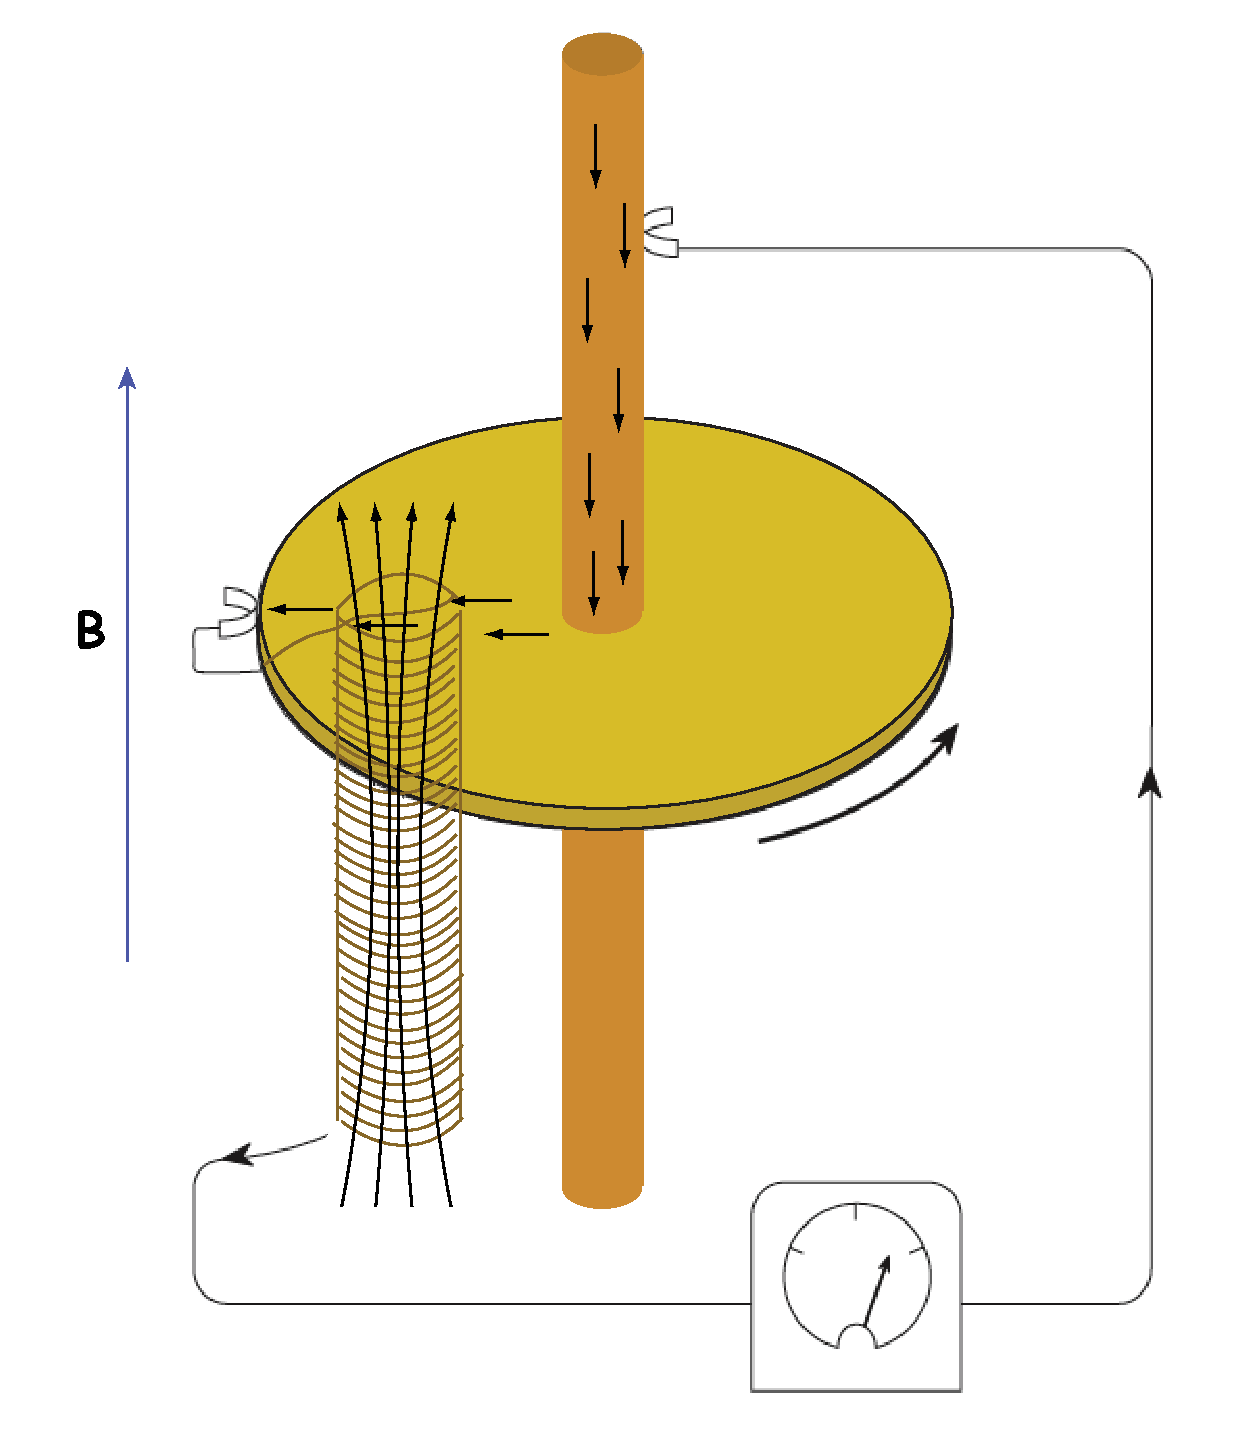
\includegraphics[width=11.5 cm]{EPSfiles/discdynamo.eps}
\caption{Self-exciting disk dynamo.   An initial field $B$ is reinforced by dynamo action.    When the conducting plate is rotated, electric charge moves perpendicular to the magnetic field setting up an electric potential between the inner conducting rod and the outer rim of the plate. If the conducting plate is connected to a coil wound such that a current produces a magnetic field in the same direction as the initial field, the magnetic field is enhanced. [AfterElsasser,  1958; redrawn from Butler, 1992.]}
\label{fig:faraday}
\end{figure}
 \nocite{elsasser58,butler92}
%\clearpage

 The 
\index{Lorentz force}%
Lorentz force is given by:

\begin{equation}
\label{eq:lorentz}
F_L= q {\bf v} \cross {\bf B },
\end{equation}

\noindent where $q$ is the electrical charge of the electrons, and $ v$ is their velocity. The Lorentz force on the
electrons is directed toward the axle of the disk and the resulting electrical current flow is toward the outside
of the disk (Figure~\ref{fig:faraday}).

Brush connectors are used to tap the electrical current from the disk, and the current passes through a
coil under the disk. This coil is cleverly wound so that the electrical current produces a magnetic induction field in the
same direction as the original field. The electrical circuit is a positive feedback system that reinforces the
original magnetic induction field. The entire disk-dynamo model is a self-exciting dynamo. As long as the
disk keeps rotating, the electrical current will flow, and the magnetic field will be sustained even if the original field disappears.

With this simple model we encounter the essential elements of any self-exciting dynamo:
\begin{enumerate}
\item A moving electrical conductor is required and is represented by the rotating copper disk.
\item An initial magnetic field is required.
\item An interaction between the magnetic field and the conductor must take place to provide reinforcement
of the original magnetic field. In the model, this interaction is the Lorentz force with the coil
acting as a positive feedback (self-exciting) circuit.
\item Energy must be supplied to overcome electrical resistivity losses. In the model, energy must be
supplied to keep the disk rotating.
\end{enumerate}


More complicated setups using two disks whose fields interact with one another generate chaotic magnetic behavior that can switch polarities even if the mechanical motion remains steady.  Certainly no one proposes that systems of disks and feedback coils exist in the Earth's core. But
interaction between the magnetic field and the electrically conducting iron-nickel alloy in the outer core can
produce a positive feedback and allow the Earth's core to operate as a self-exciting magnetohydrodynamic
dynamo. For reasonable electrical conductivities, fluid viscosity, and plausible convective fluid motions in
the Earth's outer core, the fluid motions can regenerate the magnetic field that is lost through electrical
resistivity. There is a balance between fluid motions regenerating the magnetic field and loss of magnetic
field because of electrical resistivity.
The dominant portion of the geomagnetic
field detectable at the surface is essentially dipolar with the axis of the dipole nearly parallel to the rotational axis of the Earth.   
Rotation of the Earth must therefore be a controlling factor on the time-averaged
fluid motions in the outer core.  It should also be pointed out that the magnetohydrodynamic dynamo can operate in either polarity of the
dipole. Thus, there is no contradiction between the observation of reversals of the geomagnetic
dipole and magnetohydrodynamic generation of the geomagnetic field. However, understanding the special
interactions of fluid motions and magnetic field that produce geomagnetic reversals is a major challenge.



As wise economists have long observed, there is no free lunch. The geomagnetic field is no exception.
Because of ohmic dissipation of energy, there is a requirement for energy input to drive the magnetohydrodynamic
fluid motions and thereby sustain the geomagnetic field. Estimates of the power (energy per unit
time) required to generate the geomagnetic field are about 10$^{13}$ W (roughly the output of 10$^4$ nuclear power
plants). This is about one fourth of the total geothermal flux, so the energy involved in generation of the
geomagnetic field is a substantial part of the Earth's heat budget.

Many sources of this energy have been proposed, and ideas on this topic have changed over the years.
The energy sources that are currently thought to be most reasonable are a combination of  cooling of the Earth's core with
attendant freezing of the outer core and growth of the solid inner core.  The inner core is pure iron, while the liquid outer core is some 15\% nickel (and probably has trace amounts of other elements as well).  The freezing of the inner core therefore generates a bouyancy force as the remaining liquid becomes more enriched in the lighter elements.   These energy sources are sufficient to power the   fluid
motions of the outer core required to generate the geomagnetic field.


\vskip .5 in\noindent{SUPPLEMENTAL READINGS:}
Jiles (1991), Chapter 1;   \nocite{jiles91}
Cullity (1972), Chapter 1.  \nocite{cullity72}

\vskip 24pt

\section{Problems}
{\parindent 0pt \parskip 12pt 

{\bf Problem 0}  

Before you do any of the problems in this book, you will need to know your way around a computer.  Therefore, you are strongly encouraged to consult the  \href{http://earthref.org/PmagPy/cookbook}{PmagPy website}. Follow the instructions in Chapter 1 (Installing PmagPy),  Chapter 3 (Survival computer skills), Chapter 6 (Intro to Python Programming) and Chapter 7 (Python Notebooks).     

After installing the {\bf PmagPy} package, find the directory called `Essentials\_Examples'  in the Datafiles folder and copy it to someplace on your computer with no spaces in the path.  Find your command line (for help see the  \href{http://earthref.org/PmagPy/cookbook/#command_line}{PmagPy cookbook}).   Now type on the command line:   ipython notebook   and navigate to the file `essentials\_ps\_template.ipynb' in the `Notebooks' directory of the datafiles folder.   Under the 'File' menu, select `Make a Copy' and rename your notebook `MYNAME\_ps\_1.ipynb', where MYNAME is your name (with no spaces), e.g., LimaTango.  Save this file in your homework folder.   

Notebooks are constructed as a series of `cells' which can be text or code among other things.  To view the `source' of a text cell, just click on it.  To render it, click on the `run' button (sideways triangle on the toolbar).  Text can be written in the style of LaTex to make nice looking equations, so you might want to familiarize yourself with that syntax.  To run the code in a code cell, click on the cell and then the `run' button.   Anything after a pound sign (\#) in a code block will be ignored, so this is how we comment code.  Run the code block with the comment `\# My first program.  Then make a new code block and have it print your favorite pithy phrase. 


{\bf Problem 1}

In axisymmetric spherical coordinates, $\nabla$ (the gradient operator) is given by

$$\nabla = {\partial\over { dr}} +  {\partial\over {\partial \theta}}.
$$

We also know that
$$
\H = - \nabla \psi_m,
$$

and 
that $\psi_m$ is a scalar function of position:
$$
\psi_m = {{\m \cdot \mathbf{r}}\over {4\pi r^3}}.
$$


Find the radial and tangential components of $\H$ if $\m$ is 80 ZAm$^2$, [remember that ``Z'' stands for Zeta which stands for 10$^{21}$], 
$r$ is 6 x 10$^6$ m and $\theta$ is 45$^o$.   
What are these field values in  terms of $\B$ (teslas)?

{\bf Problem 2}



a) Write an interactive python script to convert induction, moment and magnetic field quantities in cgs units to SI units.   Use the conversion factors in Table~\ref{tab:units}.    Use your program to convert the following: 

i) B = 3.5 x10$^{�5}$ G

ii) m = 2.78 x 10$^{-20}$ G cm$^3$

iii) H = 128 oe

b) Modify your script to allow conversion from cgs $=>$ SI or SI $=>$ cgs.   Rerun it to convert your answers from a) back to cgs.  

HINTS:  Review  Appendix~\ref{app:python}.    Use the {\bf raw\_input} command in Section~\ref{sect:rawinput} for getting information into a program. You will need to ask what the units of the input data will be and what output units are desired as well as what the number is.  When you read in data using {\bf raw\_input}, it comes in as a string variable and you will have to convert it to a floating point in order to change units.  

\begin{figure}[htb]
%\epsfxsize 6cm
%\centering \epsffile{EPSfiles/dipole.eps}
 \centering 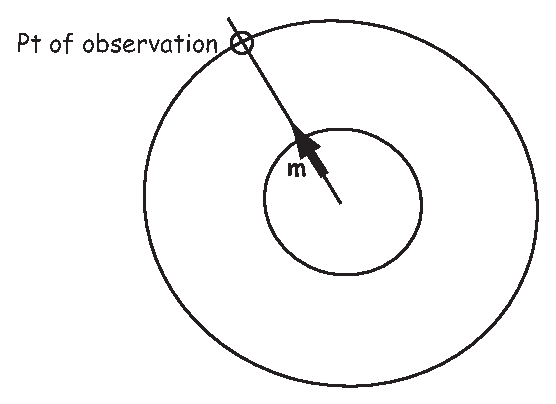
\includegraphics[width=6 cm]{EPSfiles/dipole.eps}
\caption{A magnetic dipole source (${\bf m}$) located 3480 km below the point of observation at 45$^{\circ}$ latitude.  The average radius of the Earth is 6370 km.  The field at the point of observation is directed  downward (toward the center) with a magnitude of 10 $\mu$T.  }
\label{fig:dipole}
\end{figure}


{\bf Problem 3}

 Figure~\ref{fig:dipole}  shows a meridional cross section through the Earth in the plane
of a  magnetic dipole source $m$. At the
location directly above the dipole, the field from the dipole  is directed vertically downward and has
intensity 10 $\mu$T.  The dipole source is placed at 3480 km from the center of the Earth. Assume a  mean Earth radius of  6370 km.    Adapt the
geometry of Figure~\ref{fig:mH} and the equations describing the magnetic field of a  dipole
to the model dipole in Figure~\ref{fig:dipole}.

 
a)   Calculate the magnetic dipole moment of the model dipole.  Remember to keep track of your units!   

b) 
Compare this field to the total field produced by  a centered axial magnetic dipole moment ({\it i.e.},  one that is pointing straight up and is in the center of the circles) equivalent to that of  the present geomagnetic
field ($m$ $\sim$ 80 ZAm$^2$; Z=10$^{21}$).   Assume a latitude for the point of observation of 60$^{\circ}$.  [HINT: the angle $\theta$ in Equation~\ref{eq:Vm} is the co-latitude, not the latitude.]




{\bf Problem 4}

Knowing that $B = \mu_o H$, work out the fundamental units of $\mu_o$ in SI units.  

}



